
\begin{frame}
  \frametitle{L'API OpenGL du point vue du codeur C}
  \begin{textblock}{12}(12,1.25)
    \begin{tikzpicture}
      % \draw [help lines] grid(3,2);
      % \pgfuseimage{FunnyPythonSmall}
      \node[inner sep=0pt] at (0,0) {
\includegraphics[height=10mm]{images/funny-python.png}};
      \node[draw=black, cloud callout, cloud puffs=15, aspect=2.5, cloud puff arc=120,
      callout relative pointer={(-.6,-.3)}] at (1.5,1) {void \ptr\ptr}; % absolute fails ?
    \end{tikzpicture}
  \end{textblock}
  % \frametitle{Présentation de l'API OpenGL}
  % titre ?
  API OpenGL V4.5 core~: % {\tiny (compatibility)}
  \begin{itemize}
  \item 1328 constantes {\small i.e.\ 0x1234} % {\tiny (1757)}
  \item 653 fonctions \\[.5em] % {\tiny (1044)} 
  \end{itemize}
  Paramètres~:
  \begin{itemize}
  \item type de base via typedef~: \code{(unsigned) char, short, int, float, double}
  \item pointeur~: \code{void \ptr(\ptr), char \ptr(\ptr), int \ptr, float \ptr, \ldots} \\[.5em] % * glyph
  \end{itemize}
  Return~:
  \begin{itemize}
  \item \code{unsigned char, (unsigned) int}
  \item \code{void \ptr, const unsigned char \ptr} {\tiny (quelques cas)}
  \end{itemize}
  %%%%%%%%%%
  \note{
    \begin{enumerate}
    \item 
    \end{enumerate}
  }
\end{frame}

\begin{frame}[fragile]
  \frametitle{XML API Registry~:  c'est cool!}
  \begin{tikzpicture}[remember picture, overlay, mystyle/.style={fill=red!20, opacity=1.}] % run twice
    \fill[mystyle] ($(current page.south west) + (2.4,3.3)$) rectangle +(3.2,.5);
    \node [mystyle, rectangle callout, callout relative pointer={(-3.5,-.5)}]
    at ($(current page.south west) + (10,4.5)$) {la taille est indiqué};
  \end{tikzpicture}
  \href{https://www.opengl.org/registry}{Fichier XML} définissant~: \\
  \begin{itemize}
    \item les constantes
    \item les fonctions et leurs prototypes \\
      {\tiny%
\begin{verbatim}
void glClearBufferData (GLenum target, GLenum internalformat, GLenum format, GLenum type, const void * data)

<command>
    <proto>void <name>glClearBufferData</name></proto>
    ...
    <param><ptype>GLenum</ptype> <name>format</name></param>
    <param><ptype>GLenum</ptype> <name>type</name></param>
    <param len="COMPSIZE(format,type)">const void *<name>data</name></param>
</command>
\end{verbatim}}
    \item les extensions
    \item les \textbf{versions} et leurs \textbf{profiles}
  \end{itemize}
  \centerline{\alert{$\longrightarrow$ Apporte des informations essentielles par rapport au fichier d'en-tête}}
  %%%%%%%%%%
  \note{
    \begin{enumerate}
    \item 
    \end{enumerate}
  }
\end{frame}

\begin{frame}
  \frametitle{Tous les paramètres ne ressemblent pas \ldots}
  \begin{description}[input/output via pointeur]
    \item[simple] \texttt{GLenum target} \\
      \colorG{passé par copie} \\[.5em]
      %
    \item[output par référence] \texttt{int \colorR{\ptr [1]} length} \\
      \colorG{plus d'un paramètre retourné
        cf.\ \href{http://en.wikipedia.org/wiki/X86_calling_conventions}{C calling convention}
      } \\[.5em]
      %
    \item[input/output via pointeur] \texttt{GLsizeiptr size, void \colorR{\ptr [size]} data} \\
      \colorG{la taille d'un tableau doit être indiqué en C} \\
      \attention{} \alert{XML est incomplet~: \code{size = len(p)} \textbf{ou} \code{size\_of(p)}} \\[.5em]
      %
    \item[input via pointeur] \texttt{GLsizeiptr size, \colorR{const} void \colorR{\ptr [size]} data} \\
      \colorG{\code{const} indique que le paramètre est en lecture seul} \\[.5em]
      %
    \item[pointeur complexe] \texttt{GLenum pname, GLint \colorR{\ptr [COMPSIZE(pname)]} data} \\
      \texttt{const void \ptr [COMPSIZE(format,type,width)] pixels} \\
      \colorG{la taille du tableau est calculé à partir des paramètres} \\
      \attention{} \alert{XML est incomplet~: la formule n'est pas indiqué}
  \end{description}
  %%%%%%%%%%
  \note{
    \begin{enumerate}
    \item 
    \end{enumerate}
  }
\end{frame}

\begin{frame}
  \frametitle{Architecture}
  \begin{columns}
    \begin{column}{.5\linewidth}
      \begin{center}
        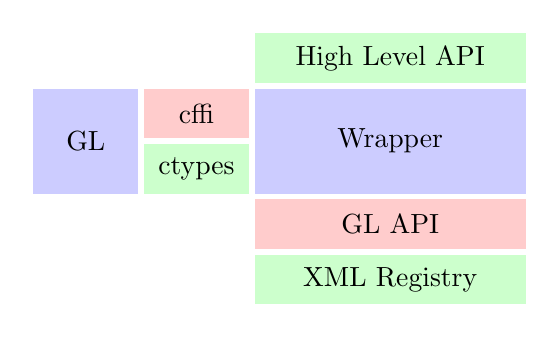
\begin{tikzpicture}[%
          base/.style={rectangle, minimum width=10em, minimum height=2em, draw=white, line width=2pt,
            anchor=south west},
          double/.style={base, minimum height=4em},
          small/.style={base, minimum width=4em}]
          % \draw [help lines] grid(3,2);
          \node[base, fill=green!20] at (0,0) {XML Registry};
          \node[base, fill=red!20] at (0,2em) {GL API};
          \node[double, fill=blue!20] at (0,4em) {Wrapper};
          \node[small, fill=green!20] at (-4em,4em) {ctypes};
          \node[small, fill=red!20] at (-4em,6em) {cffi};
          \node[double, minimum width=4em, fill=blue!20] at (-8em,4em) {GL};
          \node[base, fill=green!20] at (0,8em) {High Level API};
        \end{tikzpicture}
      \end{center}
    \end{column}
    \begin{column}{.5\linewidth}
      \begin{enumerate}
      \item l'utilisateur requiert sont API \\
        {\tiny \code{enums, commands = generate\_api(api, api\_number, profile)}}
      \item on construit le wrapper à la volé \\
        {\tiny \code{setattr(GL, enum, value)}} \\
        {\tiny \code{setattr(GL, command, class instance)}} \\
      \end{enumerate}
    \end{column}
  \end{columns}
  %%%%%%%%%%
  \note{
    \begin{enumerate}
    \item Comment est architecturé le wrapper?
    \item basé sur cffi / ctypes $\Longrightarrow$ supporte pypy
    \end{enumerate}
  }
\end{frame}

\begin{frame}[fragile]
  \frametitle{La classe Command (simplifié)}
  {\tiny
    \begin{center}
      \begin{tabular}{c|c}
        \begin{minipage}[t]{.4\linewidth}
          \centerline{Python $\longrightarrow$ C}
          \vspace{1em}
\begin{Verbatim}[commandchars=\\\{\}]
class \colorR{ParameterWrapper}():

    def __init__(self, parameter):
        ...

    def from_python(self, parameter, c_parameters):
        ...
        return to_python_converter
\end{Verbatim}
      \end{minipage}
      &
      \begin{minipage}[t]{.25\linewidth}
        \centerline{C $\longrightarrow$ Python}
        \vspace{1em}
\begin{Verbatim}[commandchars=\\\{\}]
class \colorG{ToPythonConverter}():

    def __init__(self, data):
        ...

    def __call__(self):
        ...
        return converted value
\end{Verbatim}
      \end{minipage}
    \end{tabular}
    \\[1em]
    \rule{.8\textwidth}{.5pt}
    \\[1em]
    \begin{minipage}{.8\linewidth}
\begin{Verbatim}[commandchars=\\\{\}]
class \colorB{CommandWrapper}():

    def __init__(self, wrapper, command):
        self._parameter_wrappers = [\colorR{parameter_wrapper}(parameter) for parameter in command.parameters]

    def \colorB{__call__}(self, *args, **kwargs):
        c_parameters = [None]*self._number_of_parameters

        for parameter_wrapper, parameter in zip(self._parameter_wrappers, args):
            to_python_converter = \colorR{parameter_wrapper.from_python}(parameter, c_parameters)

        return [\colorG{to_python_converter()} for to_python_converter in to_python_converters]
\end{Verbatim}
    \end{minipage}
  \end{center}}
  %%%%%%%%%%
  \note{
    \begin{enumerate}
    \item 
    \end{enumerate}
  }
\end{frame}

\begin{frame}
  \frametitle{Translation automatique des prototypes}
  \begin{description}[output par référence]
    \item[simple] \texttt{GLenum target} \\[1em]
      % \colorB{Python $\longrightarrow$ C} \\[.5em]
      % 
    \item[output par référence] \texttt{int \alert{\ptr [1]} length} \\
      \colorB{%
        % C  $\longrightarrow$ Python \\
        % retourné dans l'ordre d'apparition \\[.5em]
        \colorbox{\bgR}{int} foo(\boxG{int p1}, \boxB{int \ptr r1, int \ptr r2}) \\
        % $\longrightarrow$ \\
        \boxR{o0}, \ldots, \boxB{r1, r2} = foo(\boxG{p1})
      } \\[1em]
      % 
    \item[Pointeur Complexe]
      If
      \begin{enumerate}
      \item type = \texttt{const char \ptr}
      \item p = Numpy array~: \\
        check type if type not void \\
      \attention{} \alert{XML est incomplet~: la formule n'est pas indiqué}
      \end{enumerate}
  \end{description}
  %%%%%%%%%%
  \note{
    \begin{enumerate}
    \item 
    \end{enumerate}
  }
\end{frame}

\begin{frame}
  \frametitle{Translation automatique des prototypes~: input via pointeur}
  \texttt{GLsizeiptr size, \colorR{const} void \colorR{\ptr [size]} data} \\[.5em]
  \attention{} \alert{XML est incomplet~: \code{size = len(p)} \textbf{ou} \code{size\_of(p)}} \\
  logiquement \texttt{void} $\Longrightarrow$ \texttt{size\_of} et \texttt{float} $\Longrightarrow$ \texttt{len} \\[1em]
  \begin{columns}
    \begin{column}{.5\textwidth}
      If
      \begin{enumerate}
      \item type = \texttt{const char \ptr\ptr}~:\\
        \texttt{str(p)} ou \texttt{[str(x) for x in p]}
      \item p = Numpy array~:\\
        check type if type not void
      \item p = iterable
      \end{enumerate}
    \end{column}
    \begin{column}{.5\textwidth}
      \boxR{int} foo(\boxG{int p1}, \boxB{int \ptr s2, float \ptr p2}) \\
      % $\longrightarrow$ \\
      \boxR{o0} = foo(\boxG{p1}, \boxB{p2})
    \end{column}
  \end{columns}
  %%%%%%%%%%
  \note{
    \begin{enumerate}
    \item 
    \end{enumerate}
  }
\end{frame}

\begin{frame}
  \frametitle{Translation automatique des prototypes~: Input/Output via Pointeur}
  If \\
  % \begin{center}
  \begin{tabular}[t]{ccc}
    \numberItem{1} &
    \begin{minipage}[t]{.4\linewidth}
      type = \texttt{void \ptr}~: \\
      p = Numpy array \\
      \texttt{size = p.nbytes}
    \end{minipage} &
    \begin{minipage}[t]{.4\linewidth}
      \boxR{int} foo(\boxG{int p1}, \boxB{int s2, float \ptr p2}) \\
      % $\longrightarrow$ \\
      \boxR{o0} = foo(\boxG{p1}, \boxB{p2})
    \end{minipage}
  \end{tabular} \\[.4em]
  % 
  \begin{tabular}[t]{ccc}
    \numberItem{2} &
    \begin{minipage}[t]{.4\linewidth}
      type = \texttt{char \ptr}~: \\
      p = size
      \\ new string
    \end{minipage} &
    \begin{minipage}[t]{.4\linewidth}
      \boxR{int} foo(\boxG{int p1}, \boxB{int s2, char \ptr p2}) \\
      % $\longrightarrow$ \\
      \boxR{o0}, \boxB{p2} = foo(\boxG{p1}, \boxB{s2})
    \end{minipage}
  \end{tabular} \\[.4em]
  % 
  \begin{tabular}[t]{ccc}
    \numberItem{3} &
    \begin{minipage}[t]{.4\linewidth}
      p = Numpy array~: \\
      check type \\
      \texttt{size = p.size}
    \end{minipage} &
    \begin{minipage}[t]{.4\linewidth}
      idem \numberItem{1}
    \end{minipage}
  \end{tabular} \\[.4em]
  % 
  \begin{tabular}[t]{ccc}
    \numberItem{4} &
    \begin{minipage}[t]{.4\linewidth}
      else~: \\
      p = size \\
      new Numpy array or list
    \end{minipage} &
    \begin{minipage}[t]{.4\linewidth}
      idem \numberItem{2}
    \end{minipage}
  \end{tabular}
  % \end{center}
  %%%%%%%%%% 
  \note{
    \begin{enumerate}
    \item 
    \end{enumerate}
  }
\end{frame}

\begin{frame}[fragile]
  \frametitle{Gestion des erreurs}
\begin{verbatim}
with GL.error_checker():
  ...
\end{verbatim}
  %%%%%%%%%%
  \note{
    \begin{enumerate}
    \item 
    \end{enumerate}
  }
\end{frame}

\begin{frame}
  \frametitle{Pour aller plus loin}
  \begin{itemize}
  \item Peaufiner la GlApi
  \item Partager le code commun entre ctypes et cffi ? \\
    Ou bien conserver que cffi ?
  \item Tester plus largement le wrapper
  \item Améliorer l'interface de haut niveau
  \item Benchmark
  \end{itemize}
  %%%%%%%%%%
  \note{
    \begin{enumerate}
    \item 
    \end{enumerate}
  }
\end{frame}

%%% Local Variables: 
%%% mode: latex
%%% TeX-master: "master"
%%% End: 
